\documentclass{article}

% Language setting
% Replace `english' with e.g. `spanish' to change the document language
\usepackage[english]{babel}

% Set page size and margins
% Replace `letterpaper' with `a4paper' for UK/EU standard size
\usepackage[letterpaper,top=2cm,bottom=2cm,left=3cm,right=3cm,marginparwidth=1.75cm]{geometry}

% Useful packages
\usepackage{amsmath}
\usepackage{graphicx}
\usepackage[colorlinks=true, allcolors=blue]{hyperref}
\usepackage{xcolor}

\title{\textbf{QASST Project}}
\author{student1, first1.last1@ubbcluj.ro\\
student2, first2.last2@ubbcluj.ro\\
student3, first3.last3@ubbcluj.ro\\
student4, first4.last4@ubbcluj.ro\\
student5, first5.last5@ubbcluj.ro}
\newpage

\begin{document}
\maketitle


\tableofcontents

\newpage

\section{Software Tested}
\label{label:Software_tested}

\textcolor{blue}{Provide 2-3 sentences with details about the application under test. Any type of application is accepted (web application, mobile application, demo app from some Practice Lab, e.g., PortSwigger$->$ Academy$->$ Vulnerabilities Lab, etc.).}



\section{Approach on Security}
\label{}

\textcolor{blue}{Describe in 1-2 paragraphs the approach used to address security. \\
E.g., Defensive testing, offensive testing, or a mixed approach is accepted.
}

\section{Strategy Applied}
\label{}

\textcolor{blue}{\textit{For the offensive approach} $->$ Provide 1-2 paragraphs to describe the strategy steps used to detect vulnerabilities.\\
\textit{For the defensive approach} $->$ Detail the code that will be scanned for vulnerabilities.
}


\section{Vulnerabilities}
\label{}

\textcolor{blue}{\textit{For the defensive approach} $->$ \\(1) Use a SAST tool (e.g., Snyk) to scan the code.\\
(2) Each student that addresses the defensive approach should choose \textbf{min. 3 vulnerabilities} of different severity levels (critical, high, medium, low) to be investigated and remediated later.}

\textcolor{blue}{\textit{For the offensive approach} $->$\\
Each student that addresses the offensive approach should describe shortly \textbf{2 vulnerabilities} that will be investigated and remediated later.
}

Vulnerability 01. several details (what, how, ...) \textit{CWE-89: SQL Injection} or category \textit{A03:2021-Injection}  \cite{Vuln001} is investigated as data... [reasoning about choosing to investigate the particular vulnerability.]



\section{Aimed Assets}
\label{}

\textcolor{blue}{Describe in 1-2 paragraphs the assets that may be affected by the presence of the selected vulnerabilities.
}

\section{Affected Security Attributes}
\label{}

\textcolor{blue}{Identify the attributes from CIA triad (or CIAAN, CIANA) that are affected by the presence of the selected vulnerabilities, in relationship with the targeted assets.
}


\section{Tools Employed}
\label{}

\textcolor{blue}{Provide min. 1 paragraph with details about \textit{each} tool used to scan the code (e.g., Snyk) or to expose the selected vulnerabilities in the software (e.g., Burp Suite). 
Identify the type of the tool (SAST, DAST) and provide at least 2 benefits of each tool used.
}


\section{Test Design. Test Execution. Test Report}
\label{}

\textcolor{blue}{\textit{For the offensive approach} $->$\\
(1) For each vulnerability, \\
-- indicate/identify at least one test design technique employed to design test cases.\\
-- fill in a table with at least 3 test cases (TCs) that may expose that vulnerability.\\
(2) For each TC indicate the input, expected output, and the actual result.\\
(3) Manual testing or tool-based testing can be used (e.g., fuzzing).\\
(4) Include screenshots or tool-generated reports for the performed scan/testing.}

\textcolor{blue}{\textit{For the defensive approach} $->$\\
Include a screenshot of the report that consists of \\
(1) the report summary (\#C, \#H, \#M, \#L) and \\
(2) details about the vulnerabilities detected.}

\textcolor{blue}{Input of TCs may represent data, some SQL statements, etc. Expected output of TCs is any data or results presented to the user.}

\begin{table} [htpb]
\centering
\begin{tabular}{l|l|l|l|l}
Feature & TC ID & Input1 & Input2 & Expected Output \\ \hline
F001  &TC01 & 42 & 15 & 100\\
F001  &TC02 & 1 & -2 & 3\\
F002  &TC03 & 111 & 90 & -74
\end{tabular}
\caption{\label{tab:TCs1}TCs table.}
\end{table}

\textcolor{blue}{Table \ref{tab:TCs1} shows the TCs designed to evaluate the vulnerability AAA over F001 and F002.}


\textcolor{magenta}{This section should include test design for all team members.}


\section{Vulnerability Exploit}
\label{}

\textcolor{blue}{\textit{For the defensive approach} $->$\\
-- Imagine an attack scenario and attempt to exploit the vulnerability.\\
-- For successful attempts provide proof of the compromised assets, e.g., screenshot, data extracted, etc.}

\textcolor{blue}{\textit{For the offensive approach} $->$\\
-- Provide steps executed manually or some script that allows the exploitation of the vulnerability and compromise of the asset(s).\\
-- Include proof of the asset compromised, i.e., screenshot, data exposed/received, etc. }


\subsection{Manual Exploit}
\label{}

\textcolor{blue}{-- commands provided to extract data}

\textcolor{blue}{-- screenshots}


\subsection{Automated Exploit}
\label{}
\textcolor{blue}{- a piece of code (Python, Java, etc.) that automates the vulnerability exploited such that data is extracted/changed/updated/compromised as using/exploiting the vulnerability.}



\section{Remediation Steps}
\label{}

\textcolor{blue}{\textit{For the offensive approach} $->$\\
(1) Indicate steps to provide vulnerability remediation. E.g., piece of code, particular recommendations, etc.}

\textcolor{blue}{\textit{For the defensive approach} $->$\\
(1) Remediate/neutralize the vulnerabilities selected (3+) following the SAST tool recommendations.}\\
\textcolor{blue}{(2) For each vulnerability indicate the change in the code that is applied to fix the vulnerability. If there are multiple solutions available provide reasoning for the selected one.} \\
\textcolor{blue}{(3) Perform re-scan to prove the removal of the vulnerability, i.e., include a screenshot with a report summary (\#C, \#H, \#M, \#L) and details about the vulnerabilities re-detected.}

\section{Conclusions}
\label{}

\textcolor{blue}{Include final conclusions, lessons learned and personal considerations while working on QASSTP (3-4 paragraphs).\\
You can focus on the following aspects: type of application to be tested, amount of knowledge to use (related or not to testing), tools required to apply, team collaboration, amount of time needed to fulfill the tasks, etc.}

\section{Other sections...}

\textcolor{blue}{Please remove this section and all subsections.}
\subsection{How to include Figures}

First you have to upload the image file from your computer using the upload link in the file-tree menu. Then use the includegraphics command to include it in your document. Use the figure environment and the caption command to add a number and a caption to your figure. See the code for Figure \ref{fig:frog} in this section for an example.

Note that your figure will automatically be placed in the most appropriate place for it, given the surrounding text and taking into account other figures or tables that may be close by. You can find out more about adding images to your documents in this help article on \href{https://www.overleaf.com/learn/how-to/Including_images_on_Overleaf}{including images on Overleaf}.

\begin{figure}
\centering
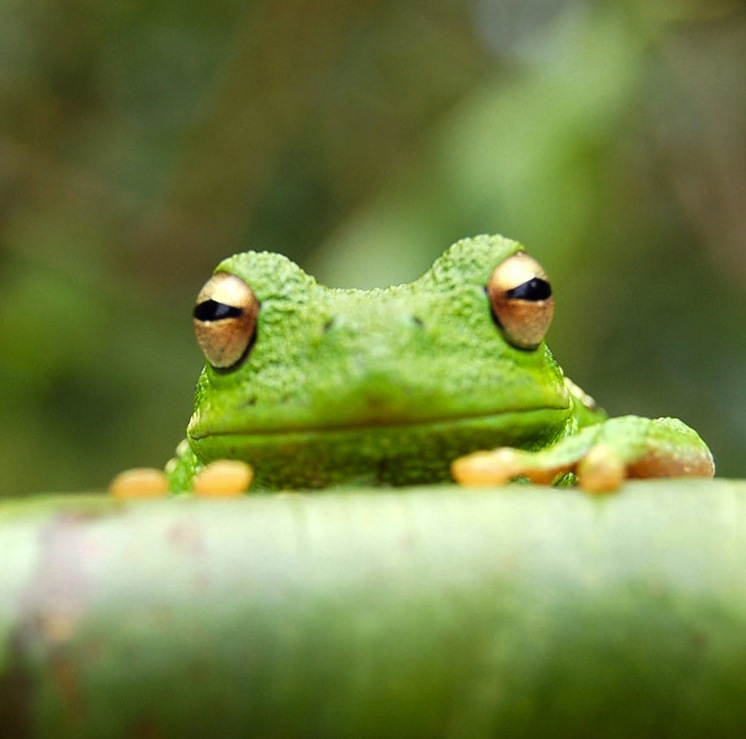
\includegraphics[width=0.25\linewidth]{Figures/frog.jpg}
\caption{\label{fig:frog}This frog was uploaded via the file-tree menu.}
\end{figure}


\subsection{How to add Citations and a References List}

You can simply upload a \verb|.bib| file containing your BibTeX entries, created with a tool such as JabRef. You can then cite entries from it, like this: \cite{greenwade93}. Just remember to specify a bibliography style, as well as the filename of the \verb|.bib|. You can find a \href{https://www.overleaf.com/help/97-how-to-include-a-bibliography-using-bibtex}{video tutorial here} to learn more about BibTeX.

If you have an \href{https://www.overleaf.com/user/subscription/plans}{upgraded account}, you can also import your Mendeley or Zotero library directly as a \verb|.bib| file, via the upload menu in the file-tree.


\bibliographystyle{alpha}
\bibliography{sample}

\end{document}